\chapter{Test Journal: Antenna transmission}\label{appendix:antennaTransmission}
\begin{table}[!h]
\begin{tabular}{l l}
\textbf{Test participants:} & Robin \& Alexander\\
\textbf{Date:}  & 29/11-2016
\end{tabular}
\end{table}

\section*{Purpose}
The purpose of this test is the measure the power transferred between the transmitting antenna and a receiving antenna, to assess the needed transmission power required for a sufficient signal to noise ratio.
\section*{Test equipment and components}
\begin{table}[!h]
	\centering
	\caption{List of measurement equipment and components}

	\begin{tabularx}{\textwidth}{lXXXX}
		Name 				& Brand	& Model & AAU-number\\ \toprule \rowcolor{lightGrey}
		Signal generator & Rohde and Schwarz & SMS 0.1 - 1040 MHz & 07927 \\ 
		Signal analyser & Rohde and Schwarz & Signal Analyser FSIQ 26 & 52766\\\rowcolor{lightGrey}
		Transmitting antenna & Pulse & W1063 & N/A\\
		Receiving patch antenna & N/A & N/A & N/A \\
	\end{tabularx}
\end{table}\label{tab_appendix:antennaTransmission}

\section*{Setup}
Diagrams of the setup for measuring the antenna transmission can be seen on Figures \ref{Appendix:fig:antennaTransSetup} and \ref{Appendix:fig:antennaTransPicture}.
\begin{figure} [!h]
    \centering
        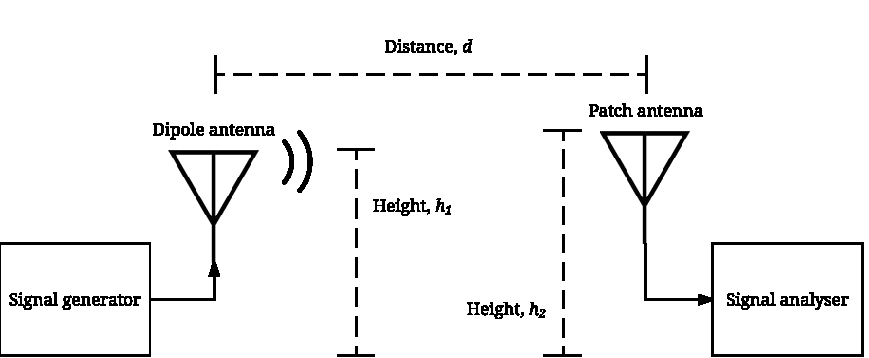
\includegraphics[width=\textwidth]{figures/test/antennaTransmission}
        \caption{Diagram of the setup for measuring the transferred signal.}
        \label{Appendix:fig:antennaTransSetup}
\end{figure}

\begin{figure} [!h]
    \centering
        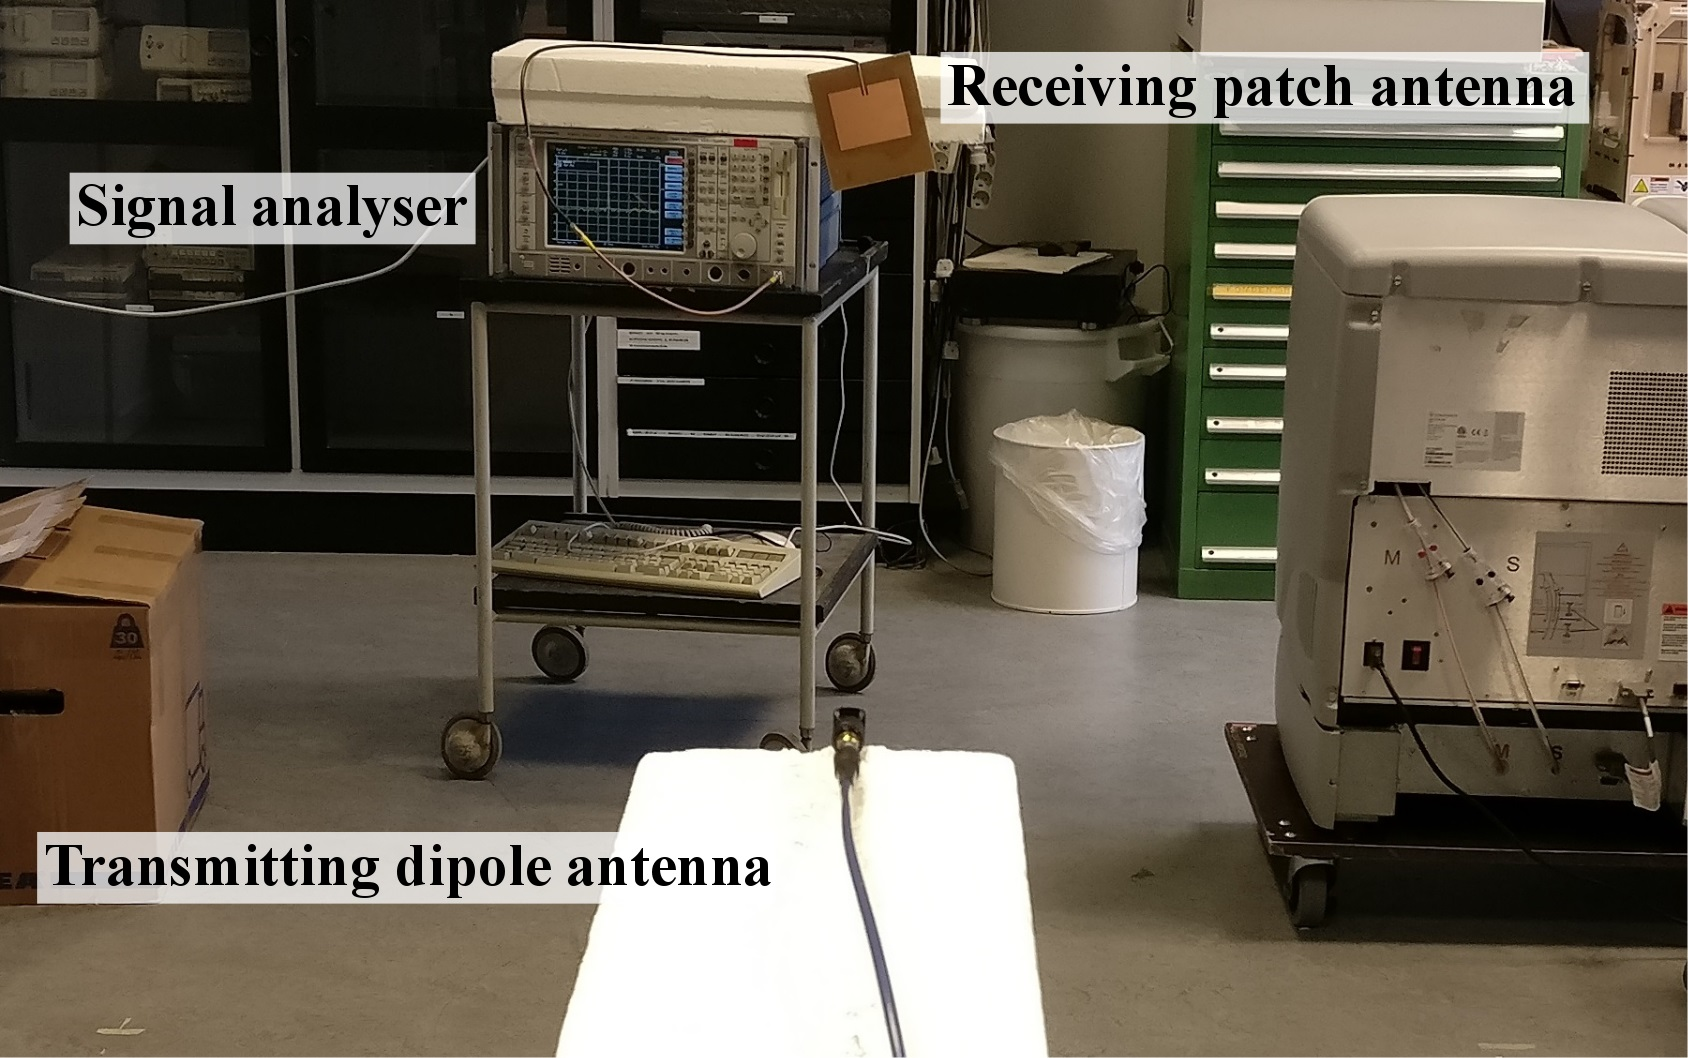
\includegraphics[width=0.8\textwidth]{figures/test/antennaTransmissionPic}
        \caption{Picture of the test setup. The transmitting antenna is attached to a signal generator, transmitting a \SI{869}{\mega\hertz} signal with a known power. The receiving antenna is attached to a signal analyser, and the received signal power and spectrum is measured.}
        \label{Appendix:fig:antennaTransPicture}
\end{figure}

\section*{Method}
Before measuring the antenna transmission, the power loss through the cables is tested, by connecting the signal generator straight to the signal analyser, and applying a signal.
Afterwards, the transmitting antenna is connected to the signal generator. The receiving antenna is connected to the signal generator. the radiation patterns of the two antennas should point in the direction of each other. 
\begin{enumerate}
\item Measure the distance from the floor, of both antennas.
\item Measure the distance between the antennas.
\item Set the transmission power to \SI{0}{\deci\belm} and frequency to \SI{869}{\mega\hertz}.
\item Measure the received power on the signal analyser.
\item Change the distance between the antennas.
\item Repeat steps 1 through 5.
\end{enumerate}

\section*{Results}
The heights of the antenna is measured as $h_1 = h_2 = \SI{1.07}{\meter}$, and the cable loss is measured as $P_{loss}=\SI{1.45}{\deci\belm}$. The rest of the results are presented in \autoref{tab_appendix:antennaTransmissionResults}
\begin{table}[!h]
	\centering
	\caption{Data of the measurement. The transmitted power $P_t$, received power $P_r$, calculated received power $P_{recal}$, the deviation $\sigma$ and the distance $d$.}\label{tab_appendix:antennaTransmissionResults}
	
\begin{tabularx}{\textwidth}{XXXXX}
	 $P_t$ [\si{\deci\belm}]& $P_r$ [\si{\deci\belm}]&$ P_{rcalc}$ [\si{\deci\belm}]& $\sigma$ [\si{\deci\belm}] & $d$ [\si{\meter}]							\\ \toprule \rowcolor{lightGrey}
		0 & \SI{-35}{}& \SI{-35.6}{}& \SI{0.6}{} &\SI{2.20}{}	\\
		0	& \SI{-38.8}{}&\SI{-37.9}{} & \SI{-1.1}{} &\SI{2.88}{}\\ \rowcolor{lightGrey}
		0 & \SI{-43}{}&\SI{-40.0}{} & \SI{-3}{} &\SI{3.65}{} 
	\end{tabularx}
\end{table}

\section*{Data processing}
The data from the test is compared with the expected results from Friis equation, without taking reflections into consideration, since it would be to complicated to calculate all the reflections of the test setup's surroundings.
If the two antennas are aligned and no reflections happen between the antennas and the attached measurement equipment, Friis equation \citep{AntennaTheoryBook} is given as \autoref{eq:appendix:antennaTransmissionFriisdB}, with gains in the form of realized gain ( $G_{realised} = G \cdot (1-\Gamma^2)$ ), where $\Gamma$ is the reflection coefficient, and units converted to a logarithmic scale. 

\begin{equation} \label{eq:appendix:antennaTransmissionFriisdB}
P_r = P_t + G_t + G_r + 20\log10\left(\frac{\lambda}{4\pi d}\right)
\end{equation}
\startexplain
\explain{$P_{r}$ is the calculated power of the received signal}{\si{\deci\belm}}
\explain{$P_{t}$ is the power of the transmitted signal}{\si{\deci\belm}}
\explain{$G_t$ is the realised gain of the transmitter antenna}{\si{\deci\bel}}
\explain{$G_r$ is the realised gain of the receiver antenna}{\si{\deci\bel}}
\explain{$\lambda$ is the wavelength of the transmitted signal in the medium, in this case air}{\si{\meter}}
\explain{$d$ is the distance between the receiver and the transmitter}{\si{\meter}}
\stopexplain

The realised gains of the antennas are given in \autoref{sec:antenna_design} as $G_r = \SI{0.03}{\deci\bel}$ and $G_t = \SI{2.49}{\deci\bel}$.
The calculated values are given in \autoref{tab_appendix:antennaTransmissionResults}.

\section*{Conclusion}
It is concluded  that a signal can be transmitted between the antennas. Friis equation gives a good estimation on the received power, even without taking reflections into considerations.




